\chapter{Literature Review}

While there are a variety NIRS devices out there, it is still very much in the research phase, though the theory behind it is well proven. Generally, there are two classes of NIRS systems used for brain imaging, LED based systems and Laser based system. All the original ones used lasers as a light source. However, as time moved on it was realized a cheaper, more convenient, safer alternative had to be found to be applicable in the clinical market. LEDs was the solution to this. They allows for a much cheaper system without the hassle of the optic cabling or the danger of lasers. Laser systems are still used today though, as they still provide advantages to LEDs. They have a much more narrow spectrum, allowing for more accurate results. They can emit a much stronger light intensity, allowing them to penetrate deeper into tissue. As such, two past NIRS devices will be discussed.

\section{Laser Based System}

Laser based NIRS system have been around for quite some time. However, there are still quite a few being designed today. One such design being designed quite recently can be seen in \cite{tor08}. The system is an Laser based multi-channel multi-wavelength NIRS system.

The advantage to on such design is it has a high acquisition frequency of 1 MHz, a very high sensitivity, a high penetration depth, a high spatial resolution, the ability to have up to 64 channels and 18 sources, and a high temporal resolution of 25 ps (higher than that of LEDs). One interesting thing about this paper is that is uses time-resolved NIRS sampling, opposed to the continuous wave NIRS sampling, most NIRS systems use. This allows the system to find the absorption and scattering coefficients individually. Continuous wave NIRS sampling can only find the combination of absorption and scattering coefficients.

The disadvantages to this system are basically the same as any Laser based system. It is highly expensive, requiring a spaghetti of optical wires (refer to Figure 2.1). The system is large an very much not portable. It is somewhat delicate, relying on Photomultiplier tubes.

\begin{figure}[htp]
\centering
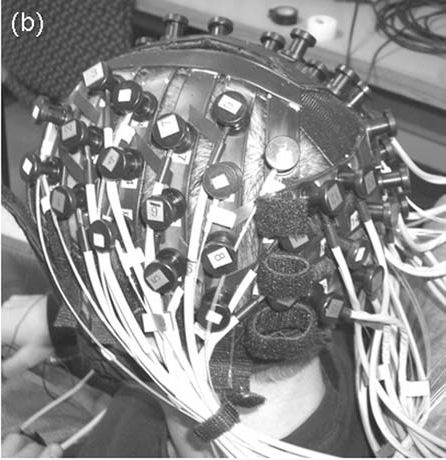
\includegraphics[width=4in]{laser.png}
\caption[Laser NIRS System]{Picture of a probe used in a Laser NIRS system. Note that this is not the system described above. \cite{fran06}}
\end{figure}

\section{The MCP II}

The MCP II is a versatile, multi-channel NIRS instrument. It was designed in order to map neuronal activation in neonatal and adult brains in response to motor, tactile, and visual stimulation. It aimed to have high SNR, good spatial sampling, and good clinical useability and ease of transportation \cite{wolf05}.

The MCP II used three LEDs to calculate the change in concentration of oxyhaemoglobin and deoxyhaemoglobin, opposed to the more common dual wavelength approach. They also used PIN photodiode's with a very large activation area, with 7.5mm$^2$, as their detectors. This is a very good idea. PIN photodiodes are especially sensitive, but with the addition of the large activation area it allows for a higher SNR \cite{wolf05}. 

The sensor designed in this system is fairly interesting. A flexible sensor that was molded with a curvature was used to fit neonatal heads as well as adults. Silicon and SMD devices were used to prevent light leakage. Transparent silicon was also placed around the photodiodes to provide two optical windows \cite{wolf05}.

The system is such designed that it is able to use 8 sensors at one time, with the ability to simultaneously measure the light intensity at two detectors. The system uses time multiplexed data acquisition with an oversampling ADC of 12-bits, to achieve a 100Hz sampling rate. Interestingly, the system is coupled to a stimulation unit that provides tactile, acoustic, and visual stimuli to the patient to accurately measure brain activity \cite{wolf05}.

The MCP II achieved very good results, obtaining a high SNR, high sensitivity, good resolution, and a good clean signal, as can be seen in Figure 2.2. Additionally, it is very convenient to have a multi-channel system that can simultaneously capture two channels \cite{wolf05}.

\begin{figure}[htp]
\centering
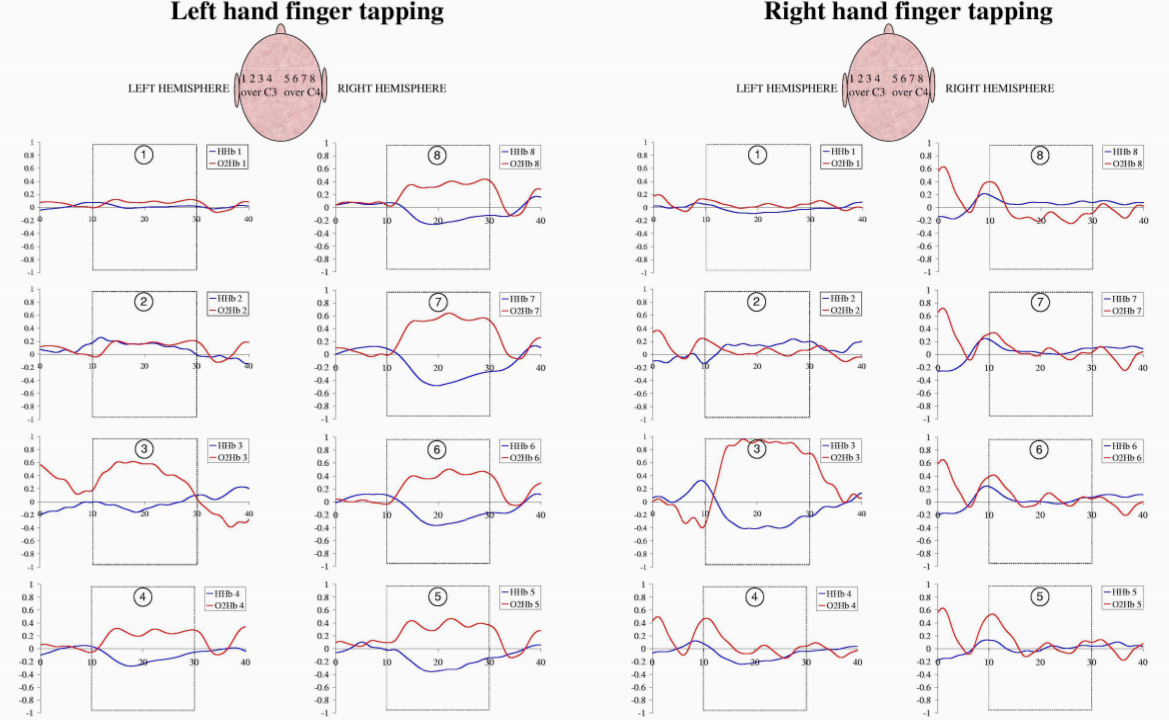
\includegraphics[width=6in]{mcp_t.png}
\caption[MCP II Measuring Motor Movement]{The MCP II measuring brain activity in the motor cortex in relation to finger tapping. "Finger tapping exercises were performed from second 10 to 30 (dotted box). The first (sensors 1-4) and the second column (sensor 5-8) measured over left and right hemisphere respectively before, during, and after left hand finger tapping. The third (sensors 1-4) and fourth column (sensor 5-8) show the left and right hemisphere during right hand finger tapping. An activation typically consists of an increase in oxyhemoglobin (O2Hb) concentration and of a decrease in deoxyhemoglobin (HHb) concentration. The higher O2 consumption in the activated area is immediately overcompensated by an increase in blood flow, which leads to the observed pattern. Both hands showed a stronger contralateral activation on the motor cortex hemisphere. The ordinates are scaled to μ mol/l." \cite{wolf05}}
\end{figure}

While, the MCP II is this projects main influence, it does have some downfalls. The system is using an unnecessarily powerful processor, running Linux, just to provide wired network communication. A simple pic18 can be used to provide network communication and be much cheaper. Additionally, the system is wired, making the system not very portable. Additionally, while the system is 'portable', it is more less transportable, rather than portable. Due to the number of channels used and the complexity of the system, it is fairly large, though comparatively small compared to Laser NIRS systems. The ideas used in the system are not original, but they successfully chose a myriad of good ideas to implement an excellent working system.

\section{Wireless Miniaturized NIRS System}

There have been similar LED based system designed that are wireless, smaller, and lighter. These designs are basically simplified designs of the MCP II,  while producing comparable results to other NIRS systems. One such design is \cite{mini08}. The main aspect of this design was to produce an lightweight, small, wireless NIRS system to minimize distress when imaging neonatal infants.

The design is simple and efficient using a dual wavelength LED design. It uses a an Silicon Labs 8051 type microcontroller connected to a Bluetooth module for communication. It is also multi-channel based system the ability to connect up to 12 channels, though only four are connected in the literature \cite{mini08}.

The sensor design, though not ideal, is unique. They grouped together multiple LEDs of the same wavelength to obtain a high integration density. Additionally, black epoxy was placed around each photodiode and LED group to prevent light contamination and leakage. The sensor placement is odd however, having two channels facing opposing directions as the other two. This is perhaps the drawback of their design \cite{mini08}.

They are able to obtain decent performance however, obtaining comparable results to that of MCP II, as can be seen in Figure 2.3.

\begin{figure}[htp]
\centering
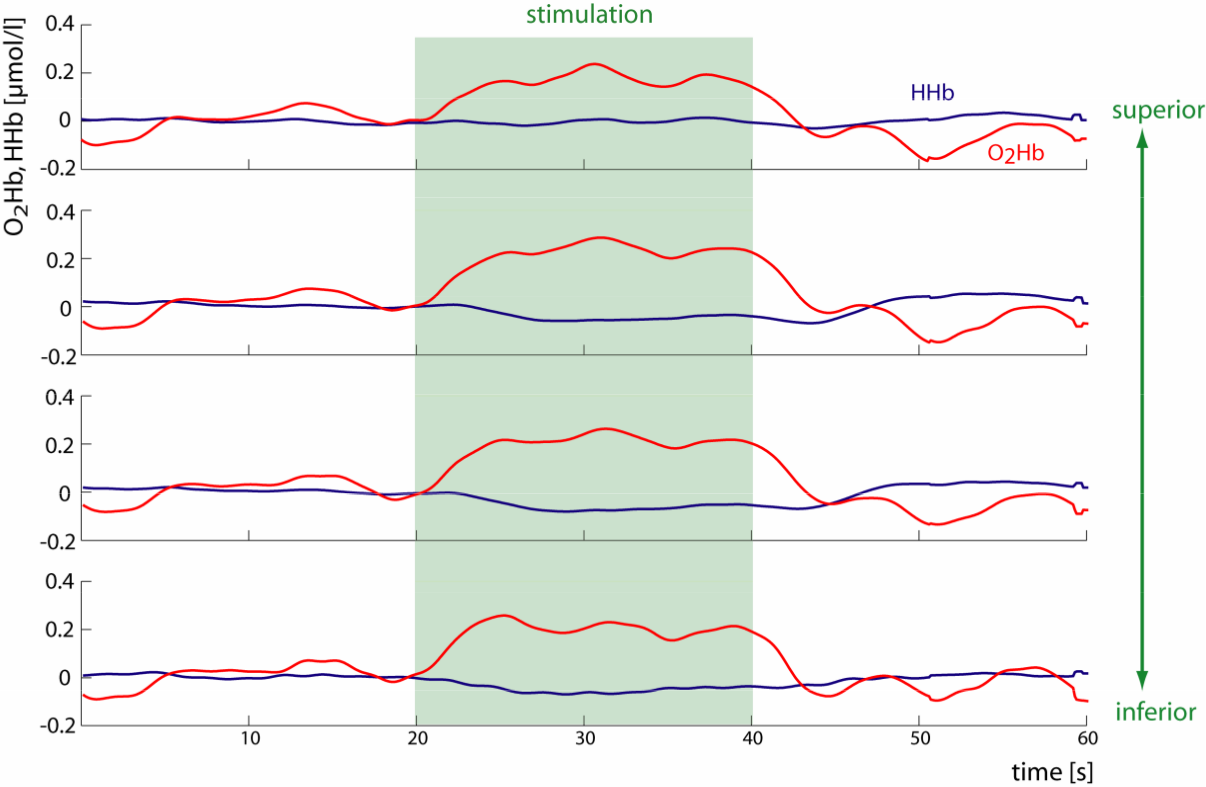
\includegraphics[width=6in]{mini.png}
\caption[Wireless Miniaturized NIRS System Measuring Motor Movement]{TheWireless Miniaturized NIRS System measuring brain activity in the motor cortex in relation to finger tapping. "Averaged hemodynamic response of the cortex to finger tapping for four source-
detector positions." \cite{mini08}}
\end{figure}